\chapter{Detecting Architectural Erosion Issues}
\label{cha:detection}

With a set of possible causes presented in Kotlin source code files from different Android projects, it is possible to define a set of rules with the help of the Android Studio IDE tools ecosystem for Architectural Erosion issues detection. We detected architectural changes in the representative set of commits and extracted different rules and patterns that could handle an architectural violation inside the MVVM architectural pattern for Android Applications. Rules could be implemented in any IDE that supports mobile development oriented to Android, like, for example, Visual Studio Code or Sublime Text (despite its constraints).


\section{UAST in Android Studio}
The Android Studio  Integrated Development Environment (IDE) is used mostly for mobile development and Android application building. Inside its ecosystem, there are a lot of built libraries, frameworks, and other programs that make the development process easier and get better performance in terms of the different non-functional requirements and architectural standards. In addition to those programs, other tools avoid committing any bad practice implementation in terms of different standards based on a specific architectural style. This tool is named linter. A linter is an integrated tool with an IDE for code insight detection and correction  (if it is possible). When we write code in Android Studio with bad code practice, its interface shows and marks a possible insight into our code. After that, we select that marker and give a possible solution for that code insight. Every rule shows its name, its description, a possible reason for the insight, and an optional code implementation solution.

This linter implementation, integrated with the Android Studio IDE, is due to the UAST structure generated by that tool. The Unified Abstract Syntax Tree (UAST) is a defined structure generated by each software project opened by the IDE that contains the AST and the Call graph structures of the source code files of that project. With this structure, we can create different semantical components (similar to the visitors components mentioned in the definitions section) that detect any pattern in different structures and code fragments inside the source code files. We can instantiate the different structures based on the Kotlin programming language grammar since there are clauses to classes and other ones. Furthermore, we can access the different attributes of each structure, like name, source code file name, or package name, and their relationships with other components. In terms of rules, we can define any customized lint check rule, and with that structure's set of Kotlin programming language and its attributes, it is possible to detect any pattern and offer any solution suggestion.

Based on the standard rules implemented in the Android Studio IDE, we can similarly define custom lint check rules for aer detection based on the insights reviewed in the representative set of commits of open-source Android projects. 

\begin{figure}[h]
    	\centering
    		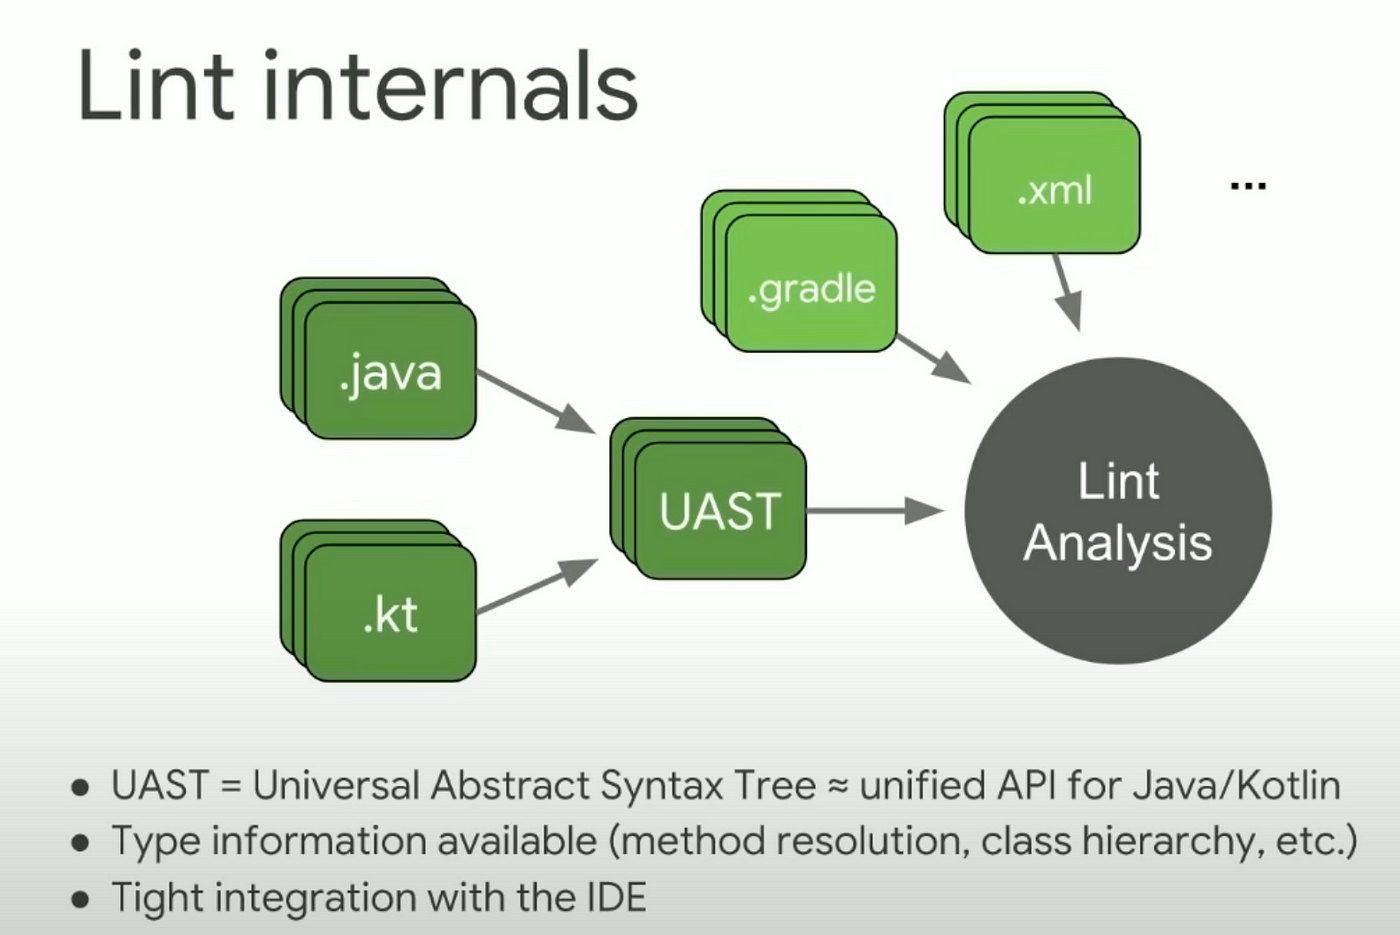
\includegraphics[scale=0.25]{/Users/juancamiloacosta/Documents/uniandes/tesis 2/thesis template repo/master-thesis-document/thesis-template/figures/uast_structure.png}
   			 \caption{Definition of Android Studio UAST structure \citet{} }
   			 \label{fig:ast}
\end{figure}

Inside the UAST structure in Android Studio, we can easily implement visitors of the abstract syntax tree. With that representation of the structure of the source code of an Android project, we can instantiate each one of them to analyze it in terms of patterns in its name, its structure, its declaration, and other features that could indicate an architectural erosion issue implemented in its structure.

\section{Rules Definition}
With the representative set extracted from the architectural erosion issues identification process, it is possible to analyze code fragments where the two judges confirmed that it could be a possible architectural violation of the original GitHub source code repository. With that, GitHub commits set and the Google architectural guidelines based on the MVVM architectural pattern \citet{}, it is possible to find troubles in architectural changes. With these architectural erosion issues, we can infer different patterns in terms of class naming, method invocation, dependency injection, and other features that could mainly affect the application performance and other significant architectural requirements inside an Android project. In the table $table_rules$, we present the different found rule sets implemented in the Kotlin programming language whose implementation could indicate an architectural erosion issue inside an Android project.

\section{AER Detector Implementation}
To implement the mentioned architectural erosion detection rules for Android applications implemented in the Kotlin programming language, we need to use the lint API toolset given by the Android Studio IDE. It is necessary to understand the tool and how we can implement its functionalities inside any Android project, in terms of version compatibility of different implemented libraries versions and automatic dependencies injection tool versions like the Gradle plugin. 

Firstly, we need to create an empty Android project. After that, we create a module that will be the main component for the custom lint check rules. We inject the main libraries to implement the linter's functionality into the project, in this case, the lint API libraries. When the project base has been implemented, we need to declare each one as an issue for the linter. Each architectural erosion rule must be implemented by stating an issue object, where we define the architectural erosion rule issue and its main attributes like name, description, category (in terms of static analysis tools like lint rules, scope rules, and other ones) severity (if the rule could indicate a severity issue, a warning issue or another category). When we declare the issue object for each rule, we need to add a visitor component that acts as a detector component to each one. To create a visitor component, we need to inject the structures that we should analyze in each pattern of each architectural erosion rule. As an example, for a bad implementation of error handling in different components and layers of an Android application, we need to analyze the try-catch structures. With UAST libraries from Android Studio, we can inject the UTryCatchStatement, which instantiates the try-catch structures found in the Android source code repository. Furthermore, we can add different filters, of which try-catch statements, we can select by name and code block structure filters.

With the base components of each architectural erosion rule, we can create a custom lint registry template for setting the custom lint check rules inside any Android project. In this file, we create the architectural erosion rules issues based on the previously created issues. After that, we implement that component as an Android library. By this, we need to inject the .jar generated file into the Android application source code; this is possible by making the .jar libraries accepted by the application in the Gradle plugin configuration file.  After that, we need to use an XML file, setting the specific name of every custom lint check rule.

With the architectural erosion rules, component creation, and the Gradle and environment parameter configuration. We execute the analysis by calling the functionality of Maven named lint. With this console command $maven --lint args$, we execute the lint rules since the default implemented lint check rules and the custom lint check rules are declared in the AER component.

\section{AER linter tool testing criteria}
Once we have the AER component with all the implemented architectural erosion rules and the parameters configuration for compatibility of each Android application, we select specific criteria for testing the implemented custom lint check rules based on the analyzed open source applications and their commit set. With the hash commit attribute, we can select a specific instant of that implementation inside the Android project source code repository and observe the custom lint check rules' effectiveness. Due to the different versions of all library ecosystems in Android development, we need to configure the test apps to set as environment variables the Java version compatibility and the Gradle plugin compatibility of the AER plugin. With these observations, we need to select specific test apps and set the environment variables for a correct lint process of each test application.
Furthermore

\subsection{Test apps selection}
With the detection process previously made,

\subsection{Building Configuration of AER Component}
